\section{Les Points cibles}
Les points cibles
% debut d'une premiere figure
%\begin{figure}[!h]
%\centering
%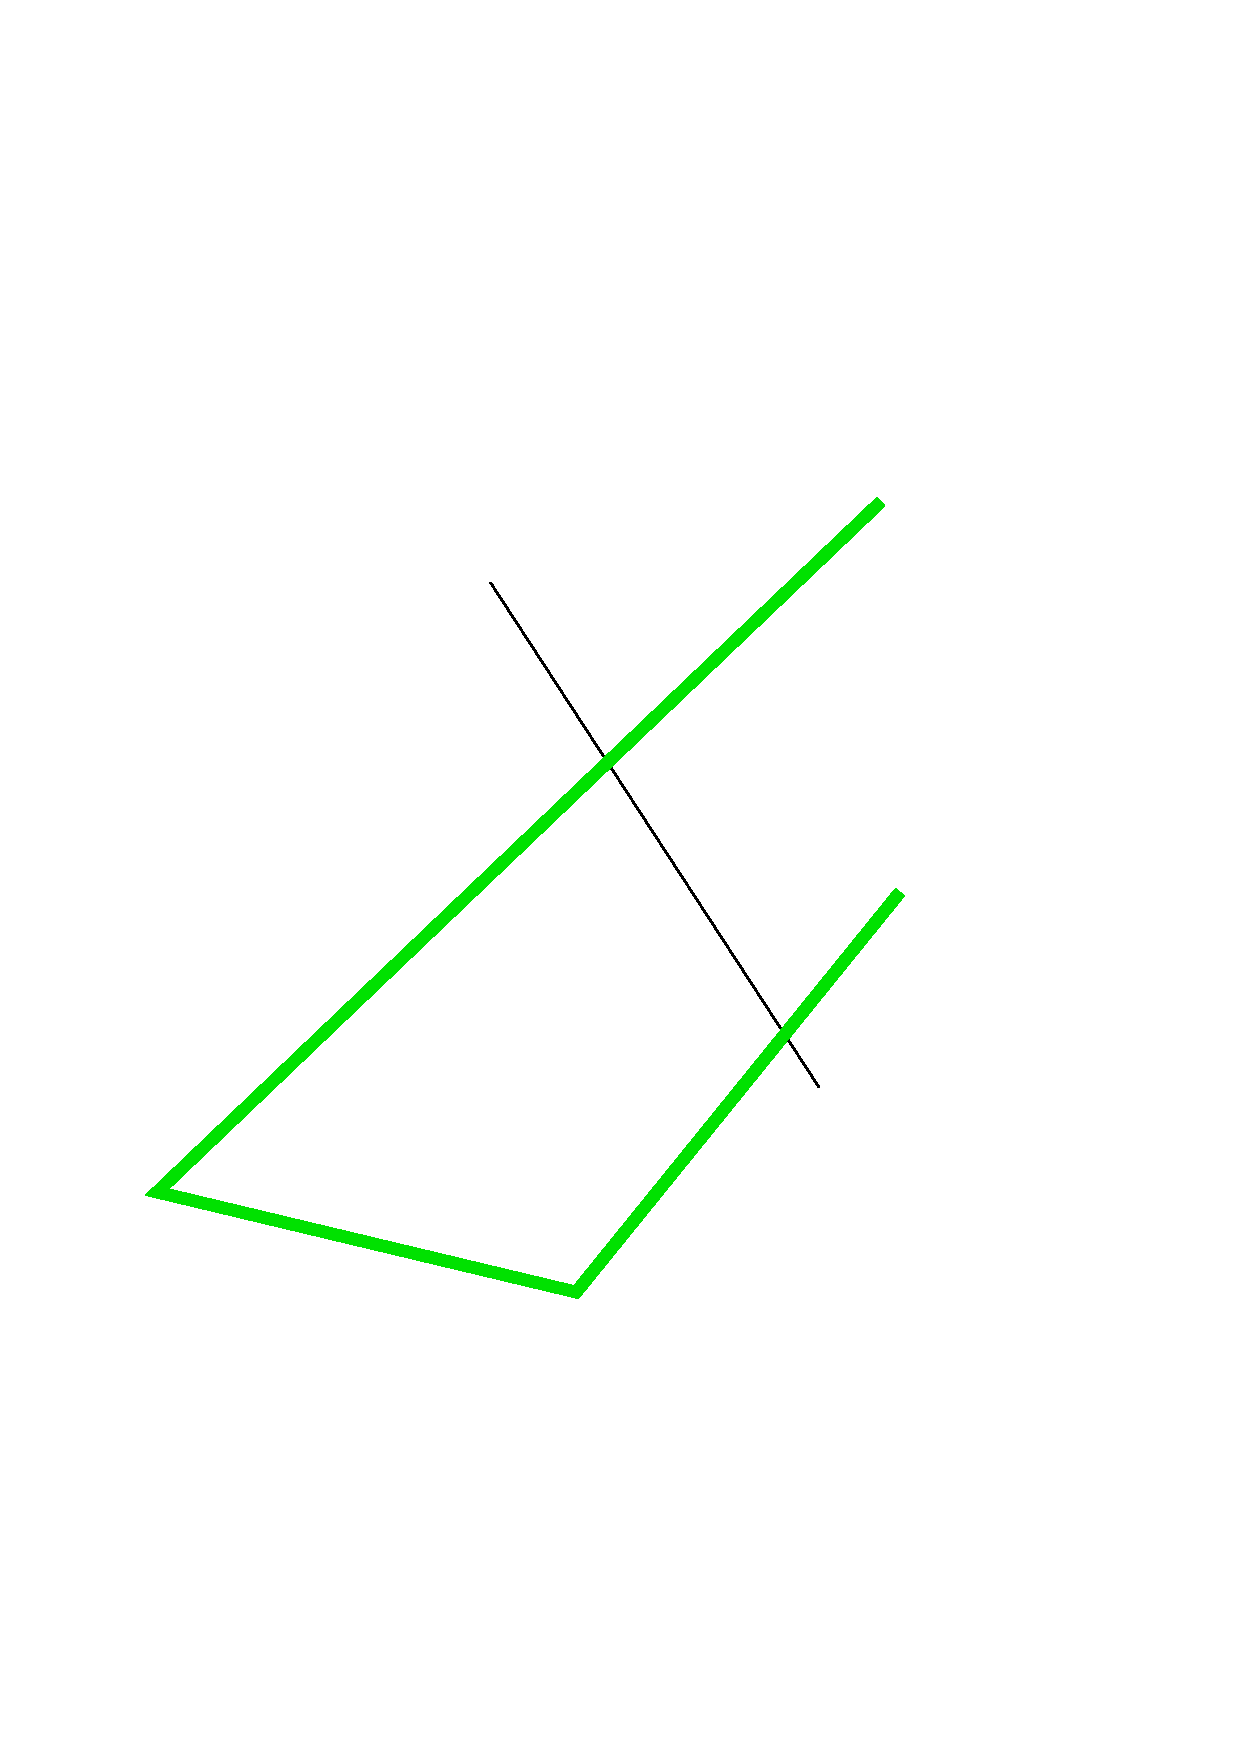
\includegraphics[width=\textwidth]{mydessin.pdf}
%\includegraphics[width=100pt]{~/f/CARTOGRAPHIE/Plans/2_Topo_EnCours/hotel_de_ville/20131210/Station\ 1/Points\ cible\ S1/P1020538.JPG}
%\includegraphics[width=100pt]{P1020538.JPG}
%\includegraphics[width=300pt,keepaspectratio=true,trim=0 0 300 300]{P1020538.JPG}
%\includegraphics[bb=0 0 2880 2160,trim=0 0 1000 1000,width=300pt,keepaspectratio=true]{P1020538.JPG}
%\includegraphics[trim=0 0 1000 1000,width=300pt,keepaspectratio=true]{P1020538.JPG}
%\includegraphics[bb=0 0 2880 2160,width=18cm,keepaspectratio=true]{P1020538.JPG}
%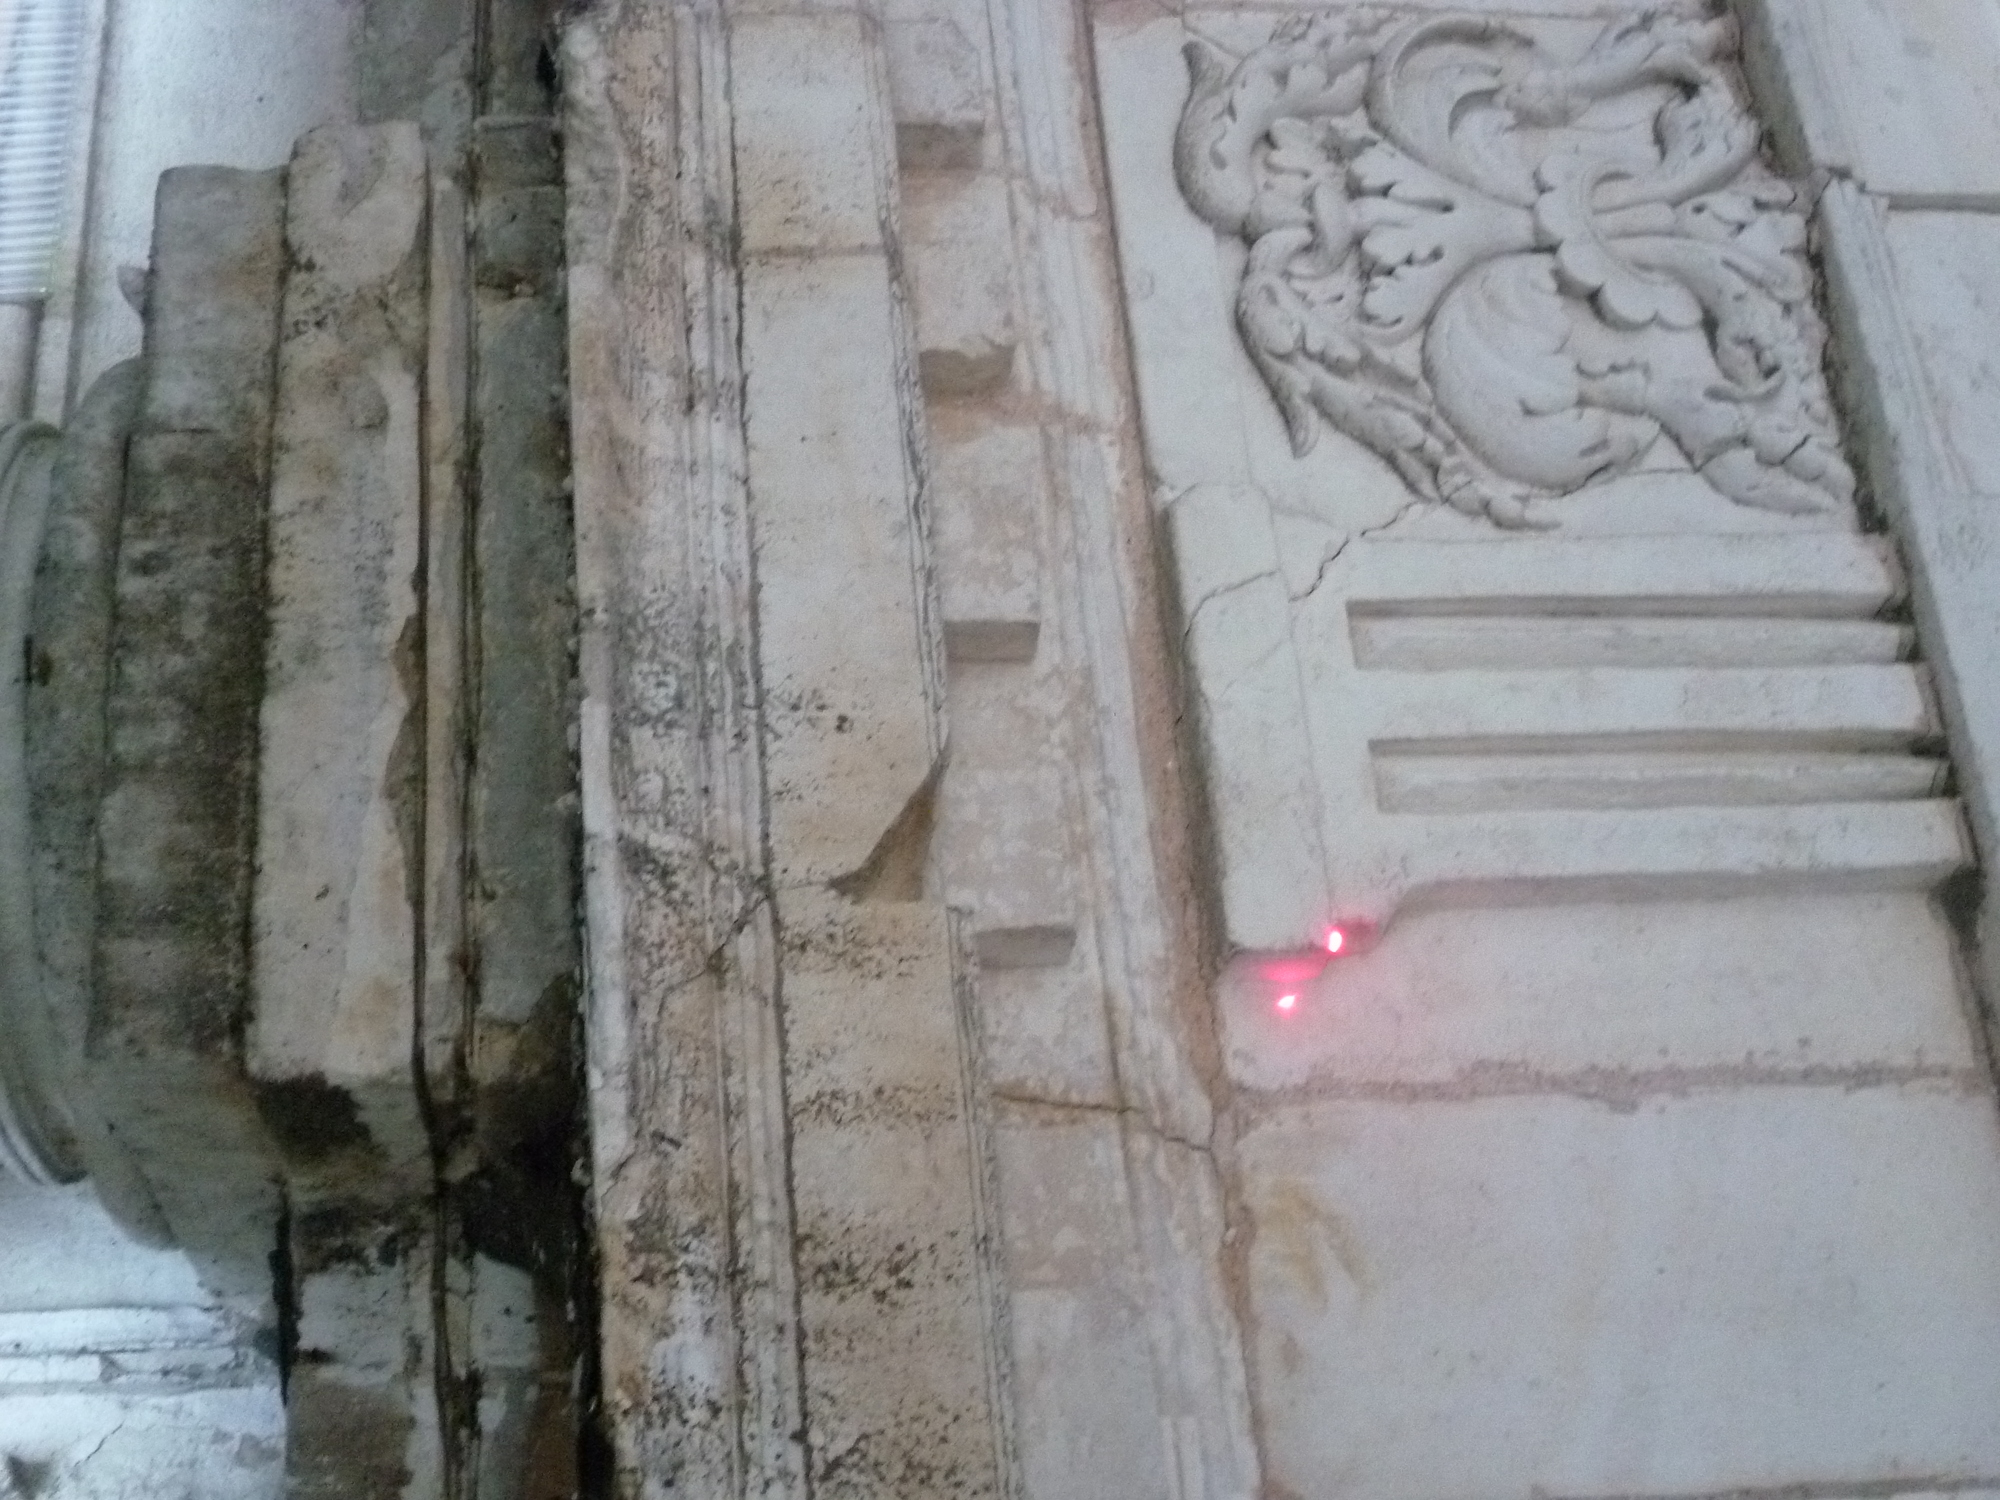
\includegraphics[bb=0 0 2880 2160,trim=0 0 400 300,width=500pt,keepaspectratio=true]{photo538.JPG}
%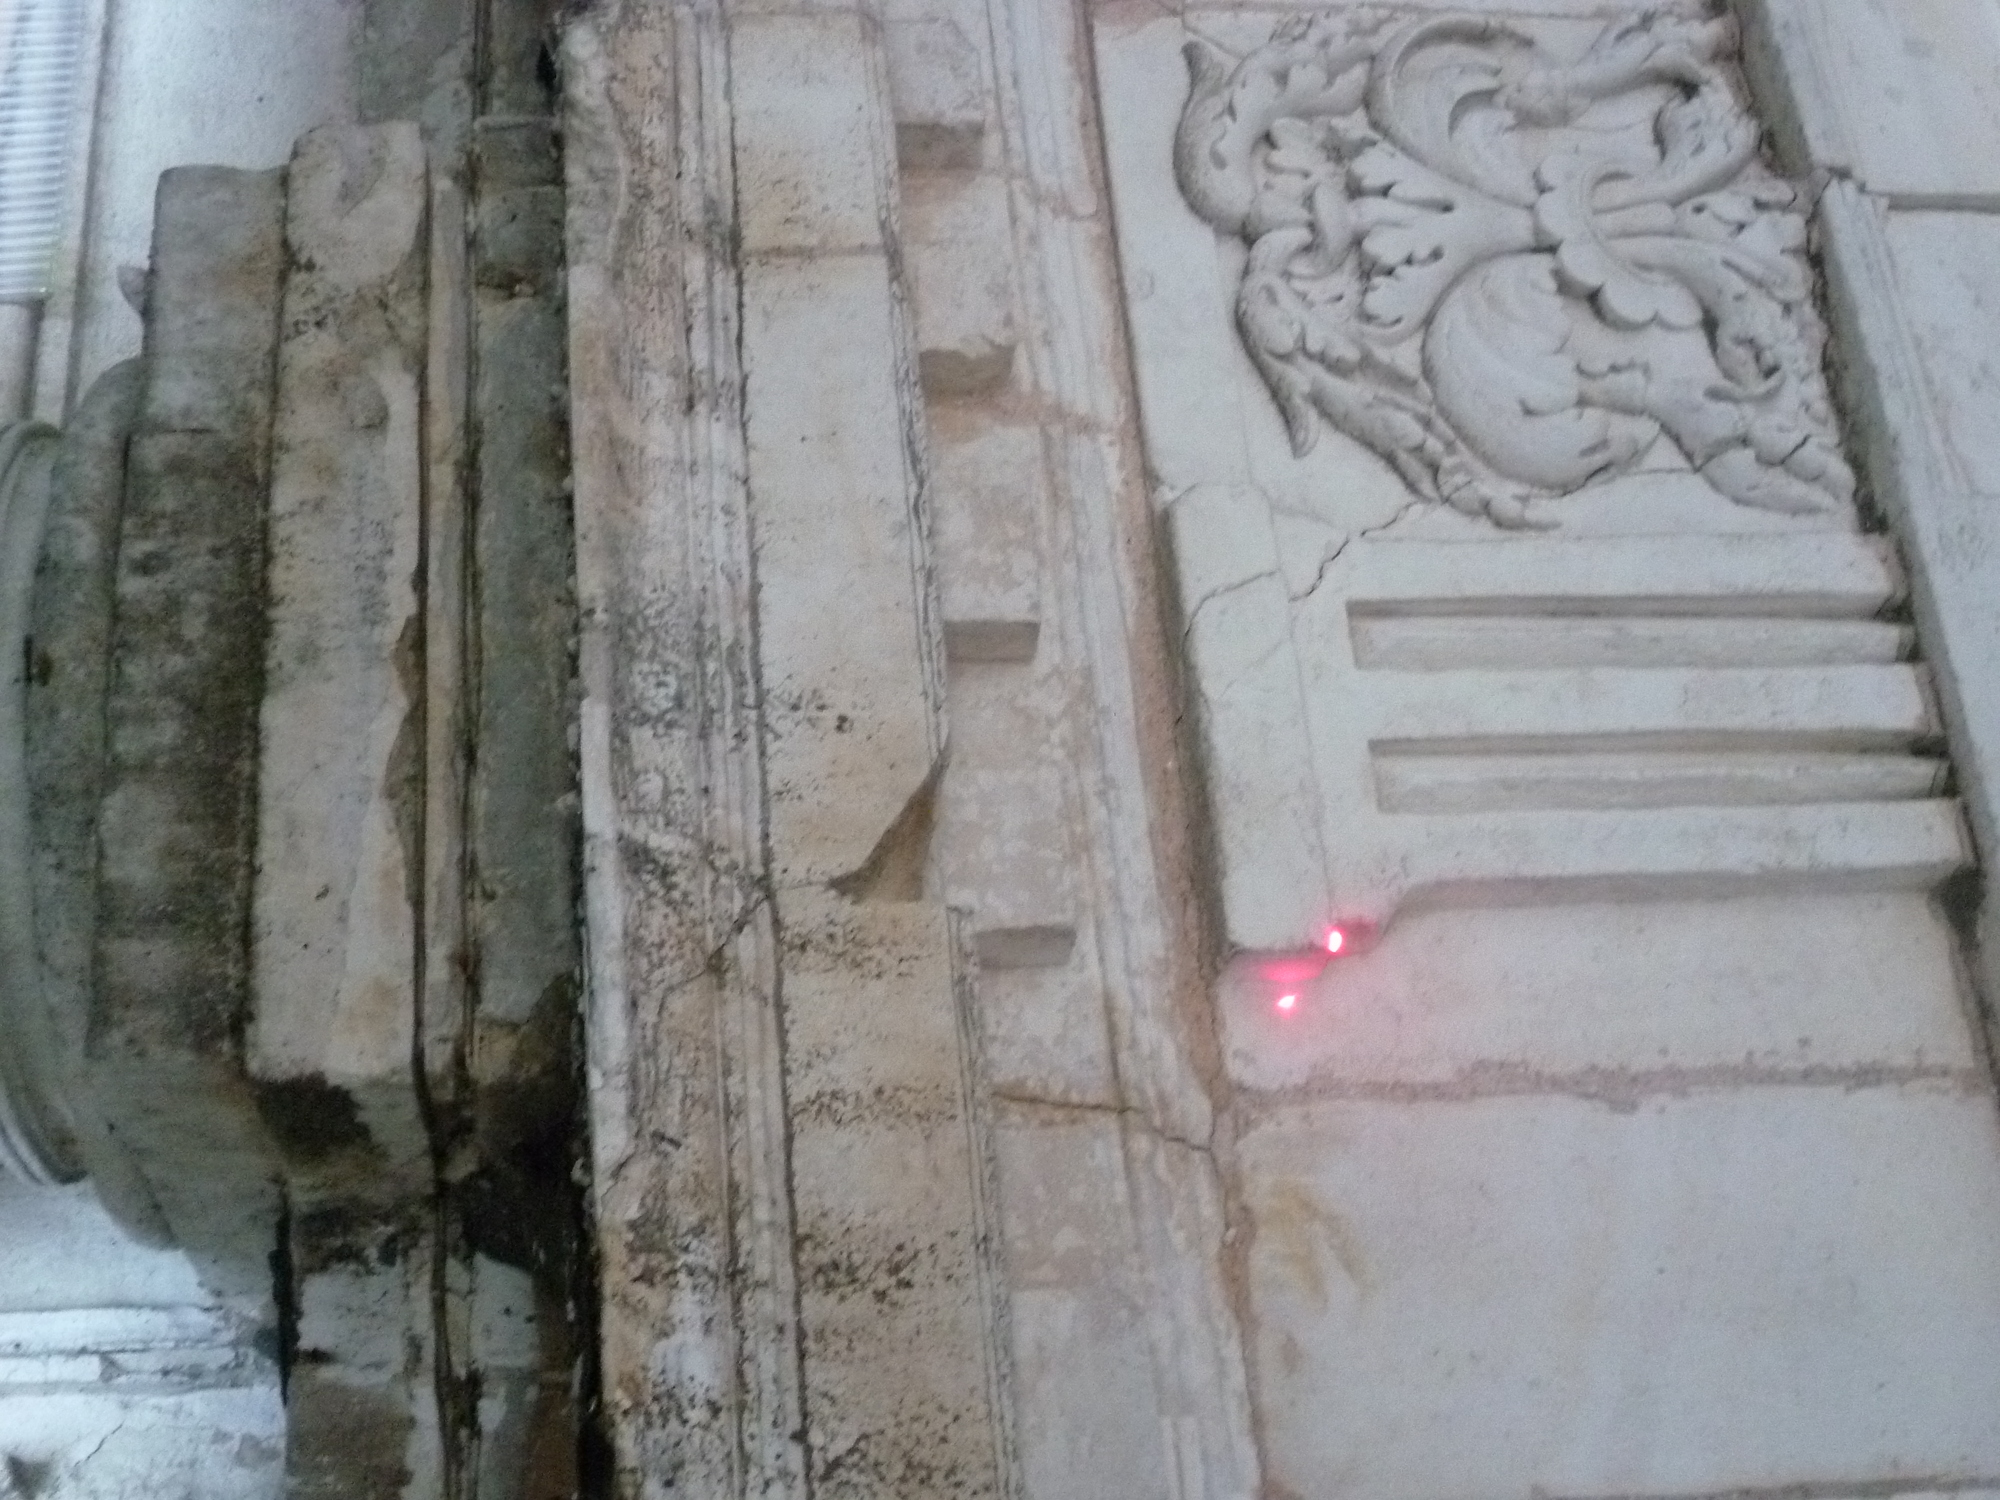
\includegraphics[trim=0 0 100 100,width=300pt,keepaspectratio=true]{photo538.JPG}
%
\includegraphics[bb=0 0 400 300,width=400pt,keepaspectratio=true]{test.jpg}
%
\includegraphics[bb=0 0 400 300,viewport=0 0 400 300,width=400pt,keepaspectratio=true]{test.jpg}
%
\includegraphics[bb=0 0 400 300,trim=0 0 399 299,width=400pt,keepaspectratio=true]{test.jpg}
%\includegraphics[trim=0 0 3000 2000,width=300pt,keepaspectratio=true]{P1020538.JPG}
%\includegraphics[width=100pt]{p1020538.jpg}
%\caption{Point 1009}
%\label{mydessin1}
%\end{figure}

